\section{Tests}

\subsection{Fest definierte Testgraphen}

\subsubsection{False}

Getestet wird zum einen mit verschiedenen fest definierten Testgraphen. Diese entsprechen bestimmten Vorgaben und sollten alle relevanten Edge Cases abdecken.\\

Für den Hierholzer Algorithmus dürfen keine gerichteten Graphen übergeben werden. Der erste Test prüft dies. Wird ein gerichteter Graph übergeben, beendet sich der Algorithmus und wirft eine Exception.\\

Der zweite zu testende Graph\ref{fig:unevenGraph} ist das Haus vom Nikolaus. Für diesen Graphen ist ein Eulerweg zu finden, allerdings kein Eulerkreis. Der Hierholzer Algorithmus schlägt hier also fehl. Beim ersten Durchlauf findet dieser den Kreis mit den Knoten A, B und C. Danach B, E, C, D. Anschließend können keine weiteren Kanten markiert werden ohne bisher markierte nochmal zu besuchen.\\
Der implementierte Algorithmus wirft in diesem Fall eine Exception.

\begin{figure}[htbp]
	\centering
		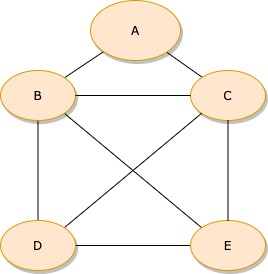
\includegraphics[width=0.25\textwidth]{Latex/Figs/unevenGraph.png}		
	\caption{Haus vom Nikolaus - ungerade Knotengerade}
	\label{fig:unevenGraph}
\end{figure}

Der dritte Graph\ref{fig:notCoherent} besteht aus zwei Komponenten. Diese hängen nicht zusammen. Folglich muss der Algorithmus auch hier abbrechen, da dies nicht erlaubt ist. Wenn nicht alle Komponenten zusammenhängen, können auch nicht alle Kanten vom einem Startpunkt aus markiert werden.

\begin{figure}[htbp]
	\centering
		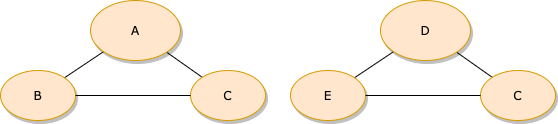
\includegraphics[width=0.60\textwidth]{Latex/Figs/notCoherent.png}		
	\caption{Ein Graph mit zwei nicht zusammenhängenden Komponenten}
	\label{fig:notCoherent}
\end{figure}

Es folgt ein Graph\ref{fig:moreNodesThanEdges} welcher mehr Knoten als Kanten besitzt. Auch in diesem Fall kann kein Eulerkreis zu finden sein. Wie im Beispiel zu sehen ist können hier der Start- und Endknoten niemals verbunden sein.

\begin{figure}[htbp]
	\centering
		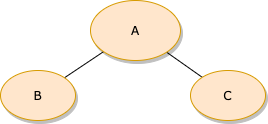
\includegraphics[width=0.30\textwidth]{Latex/Figs/moreNodesThanEdges.png}		
	\caption{Ein Graph mit mehr Knoten als Kanten}
	\label{fig:moreNodesThanEdges}
\end{figure}

\newpage

\subsubsection{True}

Der erste Test in welchem der Hierholzer durchlaufen soll testet einen leeren Graphen. Wir geben vor, dass Graphen, welche weder Knoten noch Kanten haben, ein leeres Ergebnis liefern und keine Exception werden.\\

Der nächste Graph\ref{fig:singleNode} besteht aus einem einzigen Knoten. Der Algorithmus findet keine Kante, aber einen Startknoten. Da der Startknoten hierdurch auch zum Endknoten wird, wird auch hier keine Exception geworfen und der Algorithmus läuft durch.

\begin{figure}[htbp]
	\centering
		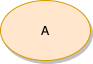
\includegraphics[width=0.15\textwidth]{Latex/Figs/singleNode.png}		
	\caption{Ein Graph mit einem einzigen Knoten}
	\label{fig:singleNode}
\end{figure}

Dieser Graph\ref{fig:fewerNodesThanEdges} erinnert an eine Sanduhr. Zusätzlich hat er hat mehr Kanten als Knoten. Im Vergleich zum Test bei welchem mehr Knoten als Kanten im Graphen waren, können in diesem Graphen zwei Eulerkreise gefunden werden. Vorausgesetzt als Startknoten werden Knoten A und C genutzt enthält der erste Eulerkreis die Knoten A, B und C - der zweite C, D und E. 

\begin{figure}[htbp]
	\centering
		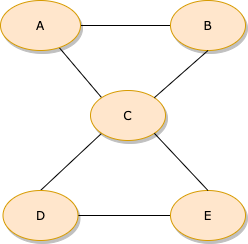
\includegraphics[width=0.3\textwidth]{Latex/Figs/fewerNodesThanEdges.png}		
	\caption{Ein Graph mehr Kanten als Knoten}
	\label{fig:fewerNodesThanEdges}
\end{figure}

Folgender Graph\ref{fig:loop} enthält eine Schleife. Auch in diesem Beispiel findet der Hierholzer Algorithmus zwei Eulerkreise. Der Knoten A ist durch eine Schleife mit sich selbst verbunden und bildet somit den ersten Eulerkreis. Der zweite Eulerkreis enthält die Knoten A, B und C.

\begin{figure}[htbp]
	\centering
		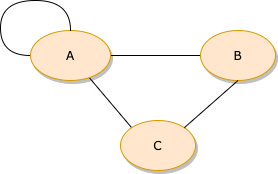
\includegraphics[width=0.35\textwidth]{Latex/Figs/loop.png}		
	\caption{Ein Graph mit einer Schleife}
	\label{fig:loop}
\end{figure}

\newpage

Der letzte statische Graph\ref{fig:multiedge} ist ein Multigraph. Dieser enthält zwei Knoten, welche durch zwei Multikanten miteinander verbunden sind. Das hier ein Eulerkreis gefunden wird ist nach den letzten Tests offensichtlich. Dieser Test prüft hauptsächlich ob die Multigraphen der Bibliothek Graphstream richtig verarbeitet werden.

\begin{figure}[htbp]
	\centering
		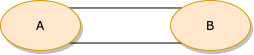
\includegraphics[width=0.3\textwidth]{Latex/Figs/twoNodesMultiEdge.png}		
	\caption{Ein Graph mehr Kanten als Knoten}
	\label{fig:multiedge}
\end{figure}